\documentclass{article}

\usepackage[utf8]{inputenc}
\usepackage{babel}
\usepackage{geometry}
\usepackage{setspace}
\usepackage{bookmark}
\usepackage{tcolorbox}
\usepackage{listings}
\usepackage{xparse}
\usepackage{xcolor}
\usepackage{hyperref}

\NewDocumentCommand{\codeword}{v}{\texttt{\textcolor{blue}{#1}}}

\lstset{language=C,keywordstyle={\bfseries \color{blue}}}

\newcommand{\HRule}[1]{\rule{\linewidth}{#1}}

\setstretch{1.2}
\geometry{
    textheight=9in,
    textwidth=5.5in,
    top=1in,
    headheight=12pt,
    headsep=25pt,
    footskip=30pt
}

\newenvironment{enfasis}
    {\begin{tcolorbox}[colback=yellow!5!white, colframe=black, width=\textwidth, sharp corners, boxrule=0.1mm]\itshape}
    {\dots\end{tcolorbox}}

% ------------------------------------------------------------------------------

\begin{document}

% ------------------------------------------------------------------------------
% Cover Page and ToC
% ------------------------------------------------------------------------------

\title{ \normalsize \textsc{}
    \\ [2.0cm]
    \HRule{1.5pt} \\
    \LARGE \textbf{\uppercase{Fundamentos de Ingeniería de Software}
    \HRule{2.0pt} \\ [0.6cm] \LARGE{Apuntes de la asignatura} \vspace*{10\baselineskip}}
}

\author{\textbf{Autores} \\
    Victor Elvira Fernández, Tomás Ruiz Rojo, Juan Horrillo Crespo \\
    Universidad de Valladolid \\
    \date{\today}}

\maketitle
\newpage

\begin{center}
    \Huge \textbf{AVISO}
\end{center}

Estos apuntes fueron creados de forma voluntaria por un grupo de estudiantes, invirtiendo tiempo, dedicación y esfuerzo para ofrecer información útil a la comunidad. Apreciamos cualquier apoyo que se nos quiera brindar, ya que nos ayuda a continuar con futuros proyectos de este tipo. \\

Si deseas colaborar en esta clase de proyectos puedes contactarnos y unirte o invitarnos a unas ricas patatas 5 salsas por el siguiente enlace:

\vfil

\begin{center}
    \href{https://www.buymeacoffee.com/ApuntesINdat}{\LARGE \textbf{Buy Me a Patatas 5 Salsas}}
    \href{https://www.buymeacoffee.com/ApuntesINdat}{https://www.buymeacoffee.com/ApuntesINdat}
\end{center}

\begin{itemize}
    \item \href{mailto:juan.horrillo22@estudiantes.uva.es}{Mail Juan Horrillo}
    \item \href{mailto:victor.elvira22@estudiantes.uva.es}{Mail Victor Elvira}
    \item \href{mailto:tomas.rojo22@estudiantes.uva.es}{Mail Tomás Rojo}
\end{itemize}

\vfil

Si has colaborado de cualquier forma te agradecemos enormemente.

\tableofcontents
\newpage

% ------------------------------------------------------------------------------

\section{Introducción a la ingeniería de software}

Segun wikipedia, se define Software como:

\begin{enfasis}
    El ``sistema formal'' de un sistema informático, que comprende el conjunto de los componentes lógicos necesarios
    que hace posible la realización de tareas específicas, en contraposición a los componentes físicos que son 
    llamados hardware.
\end{enfasis}

Para hacerlo más sencillo de entender, pero sin perder ningun tipo de detalle, para nosotros Software será:

\begin{center}
    \textbf{Los programas y toda la información asociada y materiales necesarios para soportar su instalación, 
    operación, reparación y mejora.}
\end{center}

Por tanto el software ya no tiene por que ser simplemente un programa de Java, o quizas Python, que se ejecuta 
(como los creados en asignaturas anteriores), sino que tambien puede ser un sistema formado por uno o varios 
programas, y otra gran cantidad de elementos, sean DBMS, ficheros, etc.

\noindent Siendo específicos, para crear un Software necesitaremos:
\begin{enumerate}
    \item Detallar las especificaciones.
    \item Diseñar la solución.
    \item Codificar los algoritmos.
    \item Probar el programa (o sistema).
    \item Documentar
    \item Mantener
\end{enumerate}
\noindent Esta serie de pasos es lo que se conoce como \textbf{ciclo de vida} del Software, el cual (como bien 
indica su nombre) se ``reinicia'' interminablemente durante la existencia del programa o sistema.

\noindent\rule{\textwidth}{0.4pt}

Antes de seguir indagando en los aspectos ``técnicos'' del Software, y para reflejar la importancia y complejidad 
que puede llegar a alcanzar el Software, hablemos en términos económicos y de lineas de código\dots

Segun datos de la BSA (\textit{Bussines Software Alliance}) del 2007:
\begin{itemize}
    \item El Software recoge alrededor de $1'7$ millones de empleos en EEUU.
    \item Contribuye en más de $297.000$ millones de dólares al PIB de el mismo.
    \item Tiene un crecimiento por encima del $14\%$ (¿anual?)
    \item Se invierten unos $43.000$ millones de dólares en I+D.
    \item Existen cerca de $90.000$ patentes relacionadas con el Software.
    \item Recoge un mercado de $297.000$ millones de dólares, $80.000$ millones de ellos para PC.
\end{itemize}

En la siguiente tabla se pueden observar algunos ejemplos de Software y las lineas de código que lo componen,
que a pesar de no ser totalmente lineal al tamaño del mismo (en cuanto a complejidad, inversión económica o cantidad
de personas trabajando en el), nos puede dar una idea de los monstruos con los que se trabajan:
\begin{table}[h]
    \centering
    \begin{tabular}{cc}
        \hline
        Proyecto        & \textit{LOC} (millones)   \\
        \hline
        Windows NT 3.1  & 4-5                       \\
        Windows XP      & 40                        \\
        \hline
        Linux 2.6.0     & 5.2                       \\
        Linux 2.6.35    & 13.5                      \\
        \hline
        Debian 3.0      & 104                       \\
        Debian 5.5      & 324                       \\
        \hline
        Mac OS X 10.4   & 86                        \\
        \hline
    \end{tabular}
\end{table}

\small\textit{Si, lo se, los ejemplos suenan a prehistoria, si te molesta mucho cambialos tu mismo, que a mi me da
mucha pereza actualizarlos. Buena suerte\dots}

\vspace*{2mm}

Otra posible forma de entender la magnitud de la importancia de un \textbf{buen} Software son los siguientes 
ejemplos de noticias reales:

\begin{enumerate}
    \item Recuperados $2.000$ de las $15.000$ pruebas radiológicas que se perdieron en el Hospital de Ávila
    (\href{https://www.elnortedecastilla.es/avila/201602/01/recuperados-pruebas-radiologicas-perdieron-20160201193859.html}{Fuente: El Norte de Castilla}).

    Como dijo Felix en clase, esto no se trata de los $2.000$ recuperados, se debería tratar de los otros $13.000$
    perdidos. Un fallo en el Software que gestionaba estos datos provocó pérdidas económica y humanas dificiles de 
    calcular.

    \item El Boeing 737 MAX y sus dos accidentes fatales en menos de 5 meses encienden las alertas en la aviación 
    comercial (\href{https://www.xataka.com/vehiculos/avion-boeing-737-max-sus-dos-accidentes-fatales-cinco-meses-encienden-alertas-aviacion-comercial}{Fuente: Xataca}).

    De nuevo, un fallo de Software en el sistema anti pérdidas del Boeing 737 MAX provoca pérdidas millonarias y 
    cientos de muertos por incompetencia a la hora de desarrollar Software (en este caso, se habla de que Boeing
    pudo estar pagando menos que el sueldo mínimo interprofesional a sus desarrolladores, ¡menuda ganga!). 
\end{enumerate}

\noindent Queda más que evicenciada la crucial importancia de la ingeniería de Software y las buenas prácticas que
la rodean.

\noindent\rule{\textwidth}{0.4pt}

Por supuesto que estamos de acuerdo en que el Hardware se desgasta, una bombilla se puede fundir, un condensador puede
explotar, quemar, o cualquier otra exagerada desdicha. Pero ocurre que el Software también se degrada, ¿cómo puede
ser? Una evaluación lógica, por ejemplo, \lstinline{if (numero > 0) then ...}, siempre se comportará igual, ¿no? %TODO modo code

\vspace*{2mm}

Pues no tiene por que. Una característica intrinseca al Software es que se actualiza, y muy rápidamente. Por tanto,
cosas que en el pasado funcionaban, aunque no hayan sido modificadas explicitamente, implicitamente se pueden ver
afectadas por modificaciones ajenas. A esto se le llaman habitualmente efectos secundarios.

\newpage

Es donde surje aquí el concepto de versión. Para continuar adaptandose y expandiendose a las necesidades, el
Software se actualiza al una nueva versión, maximizando las probabilidades de fallos en cada cambio.

\begin{figure}[h]
    \centering
    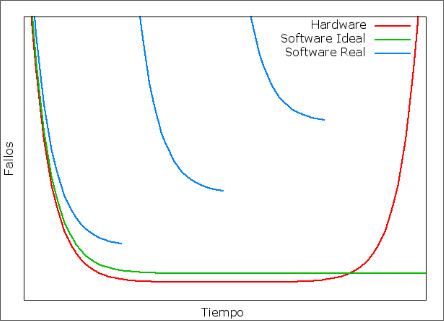
\includegraphics[width=0.7\textwidth]{assets/SoftwareFails.jpeg}
    \caption{Gráfico que ilustra el suceso}
    \label{graph:softwarefails}
\end{figure}

% ------------------------------------------------------------------------------

\newpage

% ------------------------------------------------------------------------------
% Reference and Cited Works
% ------------------------------------------------------------------------------

\begin{thebibliography}{9}
    \bibitem{diapositivas0}
    Felix Prieto, \\ \textit{Diapositivas Introducción}. \\ Universidad de Valladolid 2025
\end{thebibliography}

% ------------------------------------------------------------------------------

\end{document}

